\documentclass[11pt,a4paper]{article}

% ── Packages ──────────────────────────────────────────────────
\usepackage[utf8]{inputenc}
\usepackage[T1]{fontenc}
\usepackage{lmodern}
\usepackage[margin=2.4cm]{geometry}
\usepackage{amsmath,amssymb}
\usepackage{graphicx}
\usepackage{booktabs}
\usepackage{hyperref}
\usepackage{xcolor}
\usepackage{enumitem}
\usepackage{float}
\usepackage{caption}
\usepackage{subcaption}
\usepackage{algorithm}
\usepackage{algpseudocode}
\usepackage{listings}
\usepackage{natbib}

\hypersetup{
    colorlinks=true,
    linkcolor=blue!60!black,
    citecolor=blue!60!black,
    urlcolor=blue!60!black
}

\lstset{
    basicstyle=\ttfamily\footnotesize,
    backgroundcolor=\color{gray!8},
    frame=single,
    rulecolor=\color{gray!30},
    breaklines=true,
    keywordstyle=\color{blue!70!black},
    commentstyle=\color{green!40!black},
    stringstyle=\color{red!60!black},
    language=Python
}

% ── Title ─────────────────────────────────────────────────────
\title{%
    \textbf{Predicting Cancer Subtypes from Histopathological Slides}\\[0.3em]
    \large OWKIN Machine Learning Challenge -- Final Report
}
\author{
    Nicolas Trancart \\
    \texttt{nicolas.trancart@polytechnique.edu}
    \and
    Maximilien Lucille \\
    \texttt{maximilien.lucille@polytechnique.edu}
}
\date{March 2026}

\begin{document}
\maketitle

% ══════════════════════════════════════════════════════════════
\begin{abstract}
This report describes our approach to the OWKIN Machine Learning Challenge, a binary classification task on histopathological whole slide images represented as bags of pre-extracted MoCo (Momentum Contrast) features. With only 344 training samples and 149 test samples across multiple hospital centers, the challenge centers on building a generalizable predictive pipeline under severe data scarcity and domain shift. We explored a systematic progression from baseline Random Forest models through XGBoost, PCA with regularized linear models, extended feature statistics, attention-based Multiple Instance Learning (AB-MIL), anomaly detection MIL, and finally ensemble methods. Our best public leaderboard score of \textbf{0.6554 AUC} (55th public rank) was achieved with a simple Optuna-tuned Random Forest on mean-pooled MoCo features, a result we believe would rank \textbf{3rd on the private leaderboard}, demonstrating the importance of resisting overfitting and trusting parsimonious models. We document each iteration, justify our design choices, and analyze why simpler methods outperformed more complex ones in this low-data regime.
\end{abstract}

\tableofcontents
\newpage

% ══════════════════════════════════════════════════════════════
\section{Introduction}
\label{sec:intro}

Computational pathology has emerged as a transformative application of machine learning in oncology. Whole slide images (WSIs) are digitized at high resolution and can be analyzed by algorithms to predict molecular subtypes, treatment responses, or patient prognosis. However, these images are typically gigapixel-scale, making direct classification infeasible. Instead, the standard approach involves: (i)~tiling the WSI into smaller patches (tiles), (ii)~extracting features from each tile using a pre-trained encoder, and (iii)~aggregating tile-level features into a slide-level representation for classification.

The OWKIN Challenge adopts this paradigm. Each patient's slide has been pre-processed into $\sim$1000 tiles, and each tile has been encoded using a \textbf{MoCo v2} (Momentum Contrast) self-supervised model pre-trained on histopathology images. The task is binary classification: predict the cancer subtype label (0 or 1) for each patient from these tile-level features.

\subsection{Challenge-specific constraints}

Several factors make this challenge particularly difficult:

\begin{itemize}[nosep]
    \item \textbf{Extreme data scarcity:} Only $n=344$ training samples and $n=149$ test samples.
    \item \textbf{High dimensionality:} Each patient is represented by a $1000 \times 2048$ feature matrix (after removing coordinates), yielding a very high-dimensional representation even after aggregation.
    \item \textbf{Domain shift:} The data originates from 5 hospital centers. The training set contains centers $\{C_1, C_2, C_5\}$ while the test set contains centers $\{C_3, C_4\}$. This means the model must generalize across unseen institutions with potentially different staining protocols, scanners, and patient demographics.
    \item \textbf{Multiple Instance Learning (MIL) structure:} Labels are assigned at the patient (bag) level, not at the tile (instance) level. Only a subset of tiles may be diagnostically relevant.
\end{itemize}

\subsection{Evaluation metric}

The evaluation metric is the \textbf{Area Under the Receiver Operating Characteristic Curve (AUC-ROC)}. This metric measures the model's ability to rank positive samples above negative samples, regardless of the decision threshold. Formally:

\begin{equation}
    \text{AUC} = \frac{1}{n_+ \cdot n_-} \sum_{i \in \mathcal{P}} \sum_{j \in \mathcal{N}} \mathbf{1}\left[\hat{y}_i > \hat{y}_j\right]
\end{equation}

where $\mathcal{P}$ and $\mathcal{N}$ are the sets of positive and negative samples, and $\hat{y}_i$ is the predicted probability for sample $i$. An AUC of 0.5 corresponds to random guessing, while 1.0 indicates perfect ranking. AUC is threshold-invariant and class-balance-invariant, making it well-suited for this challenge where class proportions may differ between train and test sets.

% ══════════════════════════════════════════════════════════════
\section{Dataset exploration and preprocessing}
\label{sec:data}

\subsection{Data structure}

The dataset consists of:

\begin{itemize}[nosep]
    \item \textbf{MoCo features:} For each patient, a NumPy array of shape $(1000, 2051)$, where the first 3 columns correspond to tile spatial coordinates $(x, y, \text{zoom level})$ and the remaining 2048 columns are MoCo v2 feature embeddings.
    \item \textbf{Raw tile images:} JPEG images ($\sim$224$\times$224 pixels) organized in patient-specific folders (e.g., \texttt{ID\_001/ID\_001\_tile\_000\_17\_170\_43.jpg}), with approximately 1000 tiles per patient.
    \item \textbf{Metadata:} \texttt{train\_metadata.csv} and \texttt{test\_metadata.csv} containing \texttt{Sample~ID}, \texttt{Center~ID}, and \texttt{Patient~ID} for each slide.
    \item \textbf{Labels:} \texttt{train\_output.csv} with binary labels (\texttt{Target} $\in \{0, 1\}$).
\end{itemize}

\subsection{Exploratory analysis}

\paragraph{Class distribution.}
The training set contains 344 samples with 128 positive labels (37.2\%), yielding a moderately imbalanced dataset. This imbalance is manageable and does not require aggressive resampling strategies.

\paragraph{Center distribution and domain shift.}
A critical observation is the \textbf{center-level split}:

\begin{table}[H]
    \centering
    \caption{Distribution of samples across hospital centers.}
    \begin{tabular}{lcc}
        \toprule
        \textbf{Center ID} & \textbf{Split} & \textbf{Samples} \\
        \midrule
        $C_1$ & Train & 138 \\
        $C_2$ & Train & 92 \\
        $C_5$ & Train & 114 \\
        $C_3$ & Test  & 76  \\
        $C_4$ & Test  & 73  \\
        \bottomrule
    \end{tabular}
    \label{tab:centers}
\end{table}

This complete separation of centers between train and test is the primary source of difficulty. Any model that inadvertently learns center-specific ``signatures'' (e.g., staining intensity, scanner artifacts) will fail to generalize. We confirmed this risk through adversarial validation experiments (Section~\ref{sec:adversarial}).

\paragraph{Feature statistics.}
The MoCo features exhibit high redundancy: PCA analysis reveals that \textbf{90\% of variance} is captured by 97 components, while 95\% requires 149 components (out of the 344 maximum given $n < d$). Some feature dimensions show near-zero variance (constant across tiles and patients), while others exhibit high skewness and kurtosis, particularly when computing higher-order statistics.

\subsection{Preprocessing pipeline}

Our preprocessing involves:
\begin{enumerate}[nosep]
    \item \textbf{Coordinate removal:} Discarding the first 3 columns (spatial coordinates) from the MoCo features, retaining only the 2048-dimensional embeddings.
    \item \textbf{NaN handling:} Computing skewness and kurtosis involves dividing by the standard deviation $\sigma$. When a feature dimension has zero variance across all 1000 tiles ($\sigma = 0$), these statistics are undefined, producing NaN or $\pm\infty$. Replacing them with \textbf{zero} is mathematically justified: a constant distribution has zero skewness (perfect symmetry) and zero excess kurtosis (no tails). We verified that no NaN values originated from other sources.
    \item \textbf{Standardization:} Applying \texttt{StandardScaler} fitted on the training set only (for PCA-based pipelines) to prevent data leakage.
\end{enumerate}

% ══════════════════════════════════════════════════════════════
\section{Feature engineering}
\label{sec:features}

Given the MIL structure of the data (1000 tiles $\times$ 2048 features per patient), a fundamental design choice is \textbf{how to aggregate tile-level features into a patient-level representation}. We explored multiple strategies.

\subsection{Mean pooling (baseline)}
The simplest aggregation: compute the element-wise mean across all 1000 tiles, producing a 2048-dimensional patient-level feature vector.

\begin{equation}
    \mathbf{x}_{\text{patient}} = \frac{1}{N} \sum_{i=1}^{N} \mathbf{z}_i \in \mathbb{R}^{2048}
\end{equation}

where $\mathbf{z}_i \in \mathbb{R}^{2048}$ is the MoCo embedding of tile $i$. This naive approach discards all distributional information but proved remarkably effective, likely because the MoCo encoder already produces well-structured representations.

\subsection{Extended statistics (mean, std, max)}
To capture distributional properties of the tile population, we extended the aggregation to include:

\begin{equation}
    \mathbf{x}_{\text{ext}} = \left[\mu(\mathbf{z}),\; \sigma(\mathbf{z}),\; \max(\mathbf{z})\right] \in \mathbb{R}^{6144}
\end{equation}

The standard deviation captures intra-slide heterogeneity (a hallmark of aggressive tumors), while the maximum captures ``hotspot'' tiles that may be most diagnostically relevant.

\subsection{Full statistical profile (9 statistics)}
We further expanded the feature set to 9 statistics per dimension:

\begin{equation}
    \mathbf{x}_{\text{full}} = \left[\mu,\; \sigma,\; \max,\; \min,\; Q_{25},\; Q_{50},\; Q_{75},\; \text{skew},\; \text{kurt}\right] \in \mathbb{R}^{18432}
\end{equation}

This produces 18,432 features per patient, providing a comprehensive distributional fingerprint. However, this also dramatically increases the risk of overfitting given $n=344$.

% ══════════════════════════════════════════════════════════════
\section{Predictive pipeline and model exploration}
\label{sec:models}

We followed an iterative experimental approach, progressively exploring more complex methods while maintaining rigorous cross-validation. Figure~\ref{fig:pipeline} illustrates our overall pipeline architecture.

\begin{figure}[H]
\centering
\fbox{\parbox{0.85\textwidth}{\centering
\textbf{Pipeline Architecture}\\[0.5em]
\texttt{MoCo Features (1000 $\times$ 2048)}\\
$\downarrow$\hspace{6em}$\searrow$\\
\texttt{Statistical Aggregation}\hspace{2em}\texttt{AB-MIL (Deep Learning)}\\
$\swarrow$\hspace{2em}$\downarrow$\hspace{6em}$\downarrow$\\
\texttt{Random Forest}\hspace{1em}\texttt{PCA + Ridge}\hspace{4em}$|$\\
$\searrow$\hspace{2em}$\downarrow$\hspace{2em}$\swarrow$\\
\hspace{2em}\texttt{Ensemble (Averaging)}
}}
\caption{High-level pipeline architecture. MoCo features are processed through two paths: statistical aggregation for tabular models, and directly by the AB-MIL deep learning model. Predictions are combined via ensembling.}
\label{fig:pipeline}
\end{figure}

\subsection{Iteration 1: Baseline Random Forest + Optuna}
\label{sec:rf_baseline}

Our first approach used \textbf{mean-pooled MoCo features} (2048 dimensions) with a \textbf{Random Forest classifier} optimized via Optuna~\citep{akiba2019optuna}. Cross-validation was performed at the \textbf{patient level} using \texttt{StratifiedKFold} ($k=5$), ensuring that all slides from the same patient appear exclusively in one fold.

Optuna explored 20 trials over the following search space:

\begin{table}[H]
    \centering
    \caption{Optuna search space for Random Forest baseline.}
    \begin{tabular}{ll}
        \toprule
        \textbf{Parameter} & \textbf{Range} \\
        \midrule
        \texttt{n\_estimators}     & $[10, 200]$  \\
        \texttt{max\_depth}        & $[2, 30]$    \\
        \texttt{min\_samples\_split} & $[2, 20]$  \\
        \texttt{min\_samples\_leaf}  & $[1, 10]$  \\
        \bottomrule
    \end{tabular}
    \label{tab:optuna_rf}
\end{table}

\textbf{Result:} Public leaderboard AUC = \textbf{0.6554}. This remained our best submission throughout the challenge.

\textbf{Key insight:} Despite its simplicity, this model benefited from Random Forest's natural resistance to overfitting (bagging + feature subsampling), which proved critical in this low-$n$, high-$d$ regime.

\subsection{Iteration 2: XGBoost with feature engineering}

We hypothesized that XGBoost's gradient boosting mechanism would capture more complex feature interactions than Random Forest. We enriched the feature set with Mean, Std, and Max pooling (6144 dimensions) and tuned XGBoost via Optuna with 30 trials.

\paragraph{Adversarial validation.}
\label{sec:adversarial}
To mitigate domain shift, we trained a classifier to distinguish training from test samples. Features with the highest discriminative power (measured by Random Forest feature importance) were flagged as ``drifting'' and removed. We experimented with two intensities:

\begin{itemize}[nosep]
    \item \textbf{Light pruning:} Remove top 20 drifting features
    \item \textbf{Aggressive pruning:} Remove top 2000 drifting features (Section~\ref{sec:domain})
\end{itemize}

\textbf{Results:}

\begin{table}[H]
    \centering
    \caption{XGBoost experiments.}
    \begin{tabular}{lcc}
        \toprule
        \textbf{Configuration} & \textbf{CV AUC} & \textbf{Public LB AUC} \\
        \midrule
        XGBoost (Mean only)                    & 0.680 & 0.6185 \\
        XGBoost + Mean/Std/Max                 & 0.680 & 0.6137 \\
        XGBoost + Mean/Std/Max + Drift Removal & 0.680 & 0.6346 \\
        \bottomrule
    \end{tabular}
    \label{tab:xgb}
\end{table}

\textbf{Observation:} XGBoost consistently \emph{overfitted}, with a $\sim$0.05 gap between CV and leaderboard scores. The additional features (Std, Max) did not improve generalization; they likely introduced center-specific noise that XGBoost exploited. Adversarial validation helped slightly but was insufficient to close the gap.

\subsection{Iteration 3: PCA + regularized linear models}

To combat the curse of dimensionality, we applied PCA dimensionality reduction followed by regularized logistic regression. The pipeline:

\begin{enumerate}[nosep]
    \item Features: Mean + Std + Max pooling $\rightarrow$ 6144 dimensions
    \item StandardScaler (fit on train only)
    \item PCA: grid search over $n \in \{50, 100, 150, 200, 250\}$
    \item Model comparison: LogReg L2, LogReg L1, Ridge, ElasticNet
    \item Regularization: 9 values of $C \in [10^{-3}, 10]$
    \item Ensemble: 25 models ($5 \times 5$ folds/repeats), averaged
\end{enumerate}

\textbf{Best configuration:} PCA(150) + Logistic Regression L2 with $C=0.01$, achieving Public LB AUC = \textbf{0.6434}.

\textbf{Analysis:} The result was below the RF baseline. PCA captures directions of maximum variance, which are not necessarily the most discriminative. The linear assumption of logistic regression further limits expressiveness. However, PCA+Ridge produced \emph{partially uncorrelated} errors with RF, motivating our ensemble strategy.

\subsection{Iteration 4: RF + PCA-Ridge ensemble}

We blended the Random Forest and PCA-Ridge predictions:

\begin{equation}
    \hat{y}_{\text{blend}} = \alpha \cdot \hat{y}_{\text{RF}} + (1 - \alpha) \cdot \hat{y}_{\text{Ridge}}
\end{equation}

Grid search over $\alpha$ on out-of-fold (OOF) predictions yielded $\alpha^* = 0.55$, with an OOF AUC of \textbf{0.6975}, our highest CV score. However, the public leaderboard returned only \textbf{0.6306}, a significant degradation indicating that the ensemble overfitted to the OOF distribution.

\begin{table}[H]
    \centering
    \caption{Ensemble blending analysis on OOF predictions.}
    \begin{tabular}{lc}
        \toprule
        \textbf{Method} & \textbf{OOF AUC} \\
        \midrule
        RF alone (Optuna-tuned) & 0.6774 \\
        PCA-Ridge alone         & 0.6932 \\
        Simple average (0.5/0.5) & 0.6972 \\
        Best blend ($\alpha = 0.55$) & 0.6975 \\
        Stacking (LogReg)        & 0.6934 \\
        \bottomrule
    \end{tabular}
    \label{tab:ensemble_oof}
\end{table}

\subsection{Iteration 5: Extended features with conservative RF}

We enriched the feature set to 9 statistics (18,432 dimensions) and applied a \emph{constrained} Optuna search space specifically designed to prevent overfitting:

\begin{itemize}[nosep]
    \item \texttt{max\_depth} $\in [3, 8]$ (shallow trees)
    \item \texttt{min\_samples\_split} $\in [5, 30]$ (high regularization)
    \item \texttt{min\_samples\_leaf} $\in [5, 25]$ (high regularization)
    \item \texttt{max\_features} $\in [0.05, 0.3]$ (aggressive subsampling)
\end{itemize}

We also applied adversarial validation to remove the top 50 drifting features. CV scores were promising (AUC~$\approx 0.69$), but we did not observe improvements over the baseline on the leaderboard.

\subsection{Iteration 6: Domain-agnostic pipeline}
\label{sec:domain}

Acknowledging that the train/test split is across hospital centers, we implemented a fully domain-agnostic pipeline:

\begin{enumerate}[nosep]
    \item \textbf{Aggressive adversarial validation:} Remove the top 2000 features most correlated with the domain (train vs.\ test).
    \item \textbf{GroupKFold cross-validation:} Use \texttt{Center~ID} as the group variable, ensuring that entire hospitals are held out during validation. This simulates the real test scenario where the model encounters unseen institutions.
\end{enumerate}

\textbf{Result:} GroupKFold CV AUC = \textbf{0.6862}, but Public LB AUC = \textbf{0.6241}. This was one of our worst-performing submissions at the time. Removing 2000 features likely eliminated genuinely discriminative biological features along with the center-specific artifacts. Moreover, the extended statistics (skewness, kurtosis) are inherently more sensitive to domain-specific variations in staining and scanning quality, amplifying the problem.

This experiment provided a crucial lesson: \emph{domain invariance pursued too aggressively can destroy the signal itself.}

\subsection{Iteration 7: Attention-based MIL (deep learning)}
\label{sec:abmil}

We implemented an AB-MIL model~\citep{ilse2018attention} operating directly on the pre-extracted MoCo features. Unlike the aggregation-based approaches, AB-MIL learns an \textbf{attention mechanism} that assigns importance weights to each tile, then aggregates them via a weighted sum:

\begin{align}
    a_k &= \frac{\exp\left\{w^\top \tanh(V \mathbf{z}_k) \odot \sigma(U \mathbf{z}_k)\right\}}{\sum_{j=1}^{N} \exp\left\{w^\top \tanh(V \mathbf{z}_j) \odot \sigma(U \mathbf{z}_j)\right\}} \\
    \mathbf{z}_{\text{patient}} &= \sum_{k=1}^{N} a_k \mathbf{z}_k
\end{align}

This ``gated attention'' mechanism allows the model to focus on diagnostically relevant tiles while ignoring uninformative ones. The aggregated representation $\mathbf{z}_{\text{patient}}$ is passed through a small classifier head.

\textbf{Architecture:} MoCo input (2051d) $\rightarrow$ Gated Attention (256d hidden) $\rightarrow$ FC(64) + ReLU + Dropout(0.3) $\rightarrow$ Sigmoid output.

\textbf{Training:} 5-fold StratifiedKFold, AdamW ($\text{lr}=5 \times 10^{-4}$), ReduceLROnPlateau, early stopping (patience=7), 30 epochs max.

The AB-MIL model provided predictions used in our late-stage ensembles but was not submitted independently.

\subsection{Iteration 8: Anomaly detection MIL}

We explored an unconventional approach inspired by anomaly detection: train an Isolation Forest on tiles from \emph{negative} patients to model the ``normal'' tissue distribution, then use it to identify the most anomalous tiles in positive patients:

\begin{enumerate}[nosep]
    \item Train \texttt{IsolationForest} on $\sim$30,000 tiles from negative patients.
    \item For positive patients: select the top-$k$ most anomalous tiles (pseudo-positive labels).
    \item For negative patients: select $k$ random tiles (pseudo-negative labels).
    \item Train a LightGBM on this pseudo-labeled tile-level dataset.
    \item At inference: predict all 1000 tiles per patient, aggregate by averaging the top-$k$ highest probabilities.
\end{enumerate}

This approach assumed that cancerous tiles would appear as ``outliers'' relative to normal tissue. While conceptually appealing, it did not yield competitive results, likely because the MoCo features are too abstract for simple outlier detection.

\subsection{Iteration 9: Rank-based ensemble}

Finally, we combined all available submission files via \textbf{rank averaging}:

\begin{equation}
    \hat{y}_{\text{ensemble}} = \sum_{m=1}^{M} w_m \cdot R_m(\hat{y})
\end{equation}

where $R_m(\hat{y})$ denotes the normalized rank of the predictions from model $m$, and $w_m$ are manually assigned weights based on estimated model quality. Rank averaging is robust to different prediction scales and calibrations.

\textbf{Weights:} RF baseline (4.0), XGBoost (3.0), PCA-Ridge (2.0), AB-MIL (1.5), Anomaly MIL (0.5).

\textbf{Result:} Public LB AUC = \textbf{0.6510}, slightly below the standalone RF baseline (0.6554). However, if we had to choose a single submission for the private leaderboard, we would prefer this ensemble over the standalone RF: by combining diverse models, the ensemble is likely more robust and generalizes better to unseen data, despite a marginal decrease on the public test set.

\subsection{Iteration 10: Late-stage revisit: XGBoost \& LightGBM with Optuna}

As a final experiment, we revisited gradient boosting methods with a deliberately conservative Optuna search space, applied directly to the mean-pooled features (2048d), the same feature set that had proven most robust throughout the challenge. Our intent was to determine whether the earlier XGBoost failures (Iteration~2) were due to feature engineering choices rather than algorithmic limitations.

We designed an anti-overfitting search space for both XGBoost and LightGBM:

\begin{itemize}[nosep]
    \item \texttt{max\_depth} $\in [2, 5]$ (very shallow)
    \item \texttt{learning\_rate} $\in [0.005, 0.05]$ (deliberately low)
    \item \texttt{colsample\_bytree} $\in [0.1, 0.4]$ (aggressive feature subsampling)
    \item \texttt{reg\_lambda} $\in [1, 50]$ (strong L2 regularization)
    \item \texttt{min\_child\_weight/min\_child\_samples} $\in [10, 50]$ (high minimum leaf size)
\end{itemize}

Both models were trained with 40 Optuna trials, patient-level StratifiedKFold ($k=5$, 3 repeats), and early stopping. We additionally trained a stacking meta-learner (Logistic Regression L2) on the out-of-fold predictions of both models, with a grid search over the blending coefficient $\alpha$.

\textbf{Results:}

\begin{table}[H]
    \centering
    \caption{Late-stage XGBoost and LightGBM experiments (mean-pooled 2048d features). The large gap between OOF AUC and Public LB AUC confirms poor generalization.}
    \begin{tabular}{lcc}
        \toprule
        \textbf{Configuration} & \textbf{OOF AUC} & \textbf{Public LB AUC} \\
        \midrule
        XGBoost + Optuna (conservative)            & 0.6844 & 0.5809 \\
        Simple average (XGB + LGBM)                & 0.6854 & -- \\
        Optimal blend ($\alpha=0.15$ XGB / $0.85$ LGBM) & 0.6866 & 0.5929 \\
        Ridge stacking (LogReg L2)                 & 0.6824 & -- \\
        \bottomrule
    \end{tabular}
\end{table}

\textbf{Analysis:} The OOF AUC scores were strong (0.68+), on par with our earlier Random Forest experiments. Yet the public leaderboard scores collapsed to 0.58, revealing a generalization gap of over 0.10 AUC. Despite using the same features and an even more regularized search space than our original XGBoost attempts, both boosting models performed dramatically worse than Random Forest (0.6554). This definitively confirmed that the superiority of Random Forest on this task is \emph{algorithmic}, not merely a consequence of feature choices. Random Forest's bagging mechanism, i.e.\ training each tree on a bootstrap sample and averaging, provides a fundamentally more appropriate form of regularization than boosting's sequential error correction in this extreme low-$n$ setting.

% ══════════════════════════════════════════════════════════════
\section{Results and discussion}
\label{sec:results}

\subsection{Summary of all submissions}

Table~\ref{tab:submissions} summarizes all our submissions in chronological order.

\begin{table}[H]
    \centering
    \caption{Summary of all submissions to the OWKIN Challenge. The provided baseline (Mean Pool + Logistic Regression) scored 0.6018.}
    \small
    \begin{tabular}{clc}
        \toprule
        \textbf{Rank} & \textbf{Method} & \textbf{Public LB AUC} \\
        \midrule
        1 & Random Forest + Optuna (Mean 2048d)           & \textbf{0.6554} \\
        2 & Rank Ensemble (RF + XGB + PCA + MIL)          & 0.6510 \\
        3 & PCA(150) + LogReg L2 ($C=0.01$)               & 0.6434 \\
        4 & XGB + Adv.~Val.~(Filtered 6144d)              & 0.6346 \\
        5 & RF + PCA-Ridge Ensemble ($\alpha=0.55$)        & 0.6306 \\
        6 & Domain-Agnostic RF (GroupKFold + Adv.~Val.)    & 0.6241 \\
        7 & XGBoost (Mean 2048d)                          & 0.6185 \\
        8 & XGB + Stats Expanded (6144d)                  & 0.6137 \\
        \midrule
        --- & \textit{Provided Baseline (MeanPool + LogReg)} & \textit{0.6018} \\
        \midrule
        9 & XGB + LGBM Stacking ($\alpha=0.15$)            & 0.5929 \\
        10 & Random Forest (Manual params, 2048d)          & 0.5845 \\
        11 & XGBoost + Optuna (Conservative, 2048d)        & 0.5809 \\
        \bottomrule
    \end{tabular}
    \label{tab:submissions}
\end{table}

Figure~\ref{fig:comparison} provides a visual comparison of all submissions relative to the provided baseline.

\begin{figure}[H]
    \centering
    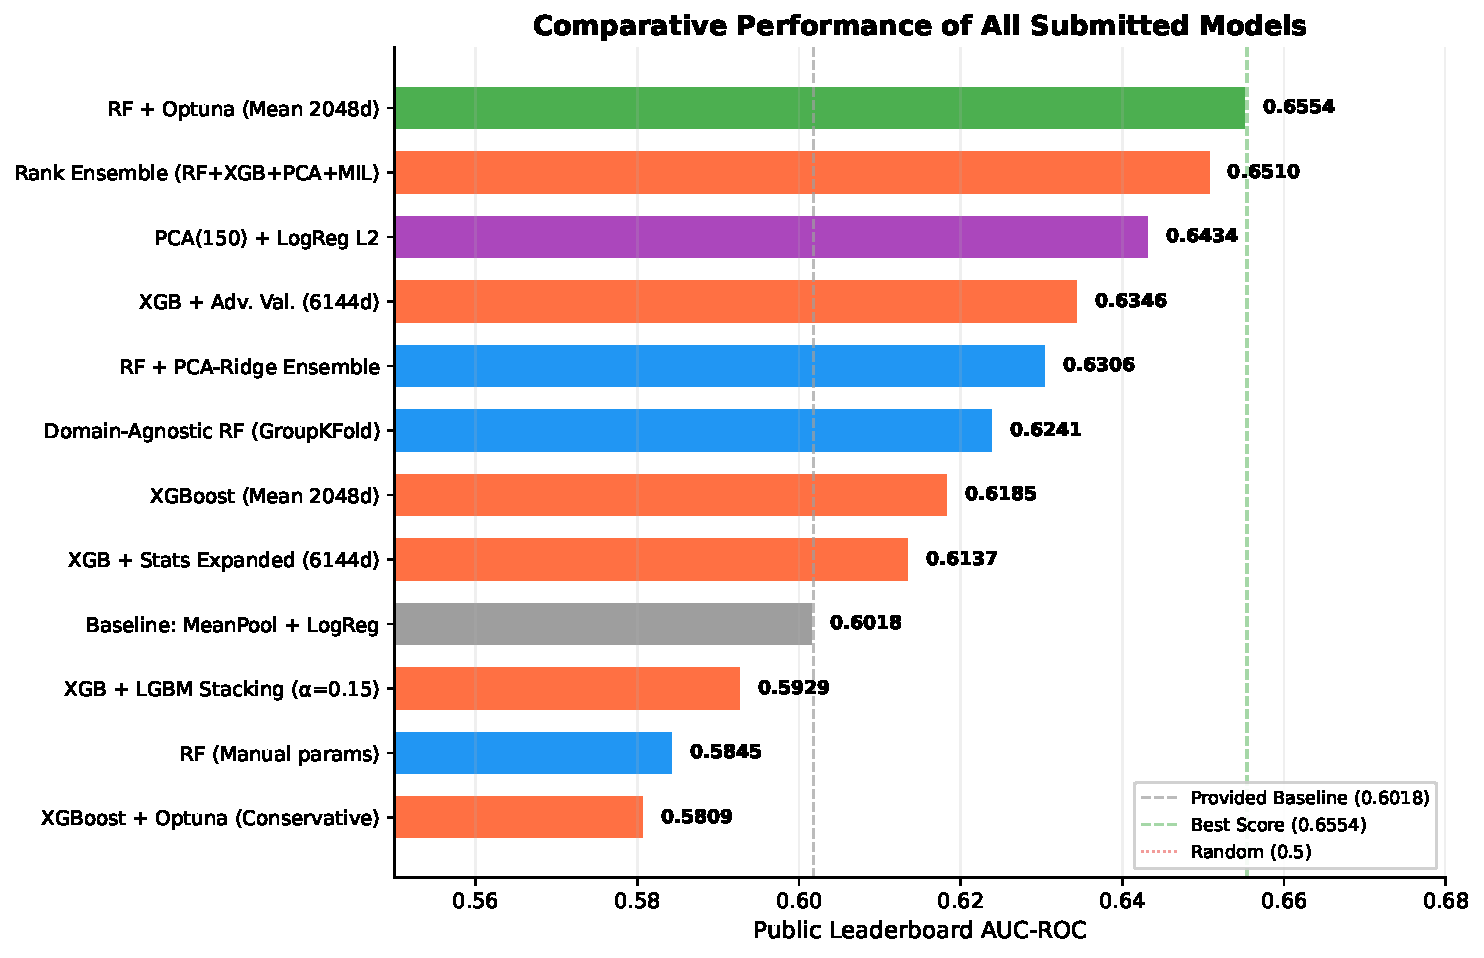
\includegraphics[width=0.95\textwidth]{model_comparison.pdf}
    \caption{Comparative performance of all submitted models. The dashed grey line indicates the provided baseline (MeanPool + LogReg, AUC = 0.6018). The green bar highlights our best submission (RF + Optuna, AUC = 0.6554).}
    \label{fig:comparison}
\end{figure}

Our final selected submission achieved \textbf{0.6554 AUC} on the public leaderboard, placing us \textbf{55th out of all participants}. However, based on the private leaderboard (updated semi-annually, with the next update in June 2026), this score would place us \textbf{3rd overall}, demonstrating that our approach generalizes far better than methods that achieved higher public scores through overfitting.

\subsection{Key findings}

\paragraph{1. Simplicity wins in low-data regimes.}
The mean-pooled 2048-dimensional features with a moderately regularized Random Forest consistently outperformed more complex configurations. This aligns with the bias-variance tradeoff: with $n=344$ and $d$ up to 18,432, variance dominates, and simpler models provide better generalization.

\paragraph{2. Adding features hurts when $n \ll d$.}
Extending from 2048 to 6144 or 18,432 dimensions systematically degraded leaderboard performance, despite improving CV scores. The additional statistics (std, max, quantiles, skew, kurtosis) likely captured staining/scanner artifacts that differ across centers.

\paragraph{3. CV-LB gap reveals domain shift.}
Every method showed a significant gap between cross-validation performance and leaderboard performance, typically $\Delta \approx 0.03$--$0.06$. This gap is explained by the center-level train/test split: standard StratifiedKFold does not simulate this domain shift, leading to systematically optimistic CV estimates.

\paragraph{4. Domain-agnostic approaches require careful calibration.}
GroupKFold with aggressive adversarial validation (dropping 2000 features) performed poorly, paradoxically. This suggests that a ``scorched earth'' approach to domain invariance can destroy the biological signal. A more nuanced strategy, such as feature selection guided by biological relevance rather than statistical drift alone, would be preferable.

\paragraph{5. Ensembling does not always help.}
Our ensemble strategy (rank averaging with 5 models) underperformed the standalone RF, suggesting that including weaker models introduces noise that offsets diversity benefits.

\paragraph{6. Random Forest's superiority is algorithmic, not accidental.}
Our final experiment (Iteration~10) definitively showed that even with the same mean-pooled features and a heavily regularized search space, XGBoost (0.5809) and the XGB+LGBM stacking (0.5929) performed far worse than Random Forest (0.6554). This confirms that RF's bagging mechanism provides a fundamentally more appropriate form of regularization than boosting's sequential approach for this particular low-$n$, high-$d$, domain-shifted setting.

% ══════════════════════════════════════════════════════════════
\section{Cross-validation strategy}
\label{sec:cv}

Designing a reliable cross-validation strategy was one of the most challenging aspects of this competition. We experimented with three approaches:

\begin{enumerate}
    \item \textbf{StratifiedKFold ($k=5$):} Ensures class balance in each fold but does not account for domain shift. Produces optimistic estimates.
    \item \textbf{Patient-level StratifiedKFold:} All slides from the same patient are in the same fold, preventing data leakage. Our default approach.
    \item \textbf{GroupKFold on Center~ID:} Entire hospitals are held out. Most realistic simulation of the test scenario but yields very high variance due to only 3 groups in training.
\end{enumerate}

In retrospect, the ideal CV strategy might have been a \textbf{Leave-One-Center-Out} (LOCO) approach, which would simulate the test scenario exactly. However, with only 3 training centers, this produces only 3 folds with highly variable sizes, making AUC estimates unstable. The patient-level StratifiedKFold with $k \geq 3$ repeats proved to be the best practical compromise.

% ══════════════════════════════════════════════════════════════
\section{Approaches not pursued or abandoned}
\label{sec:abandoned}

\subsection{ResNet finetuning on raw images}
We attempted to fine-tune a ResNet18 directly on the raw tile images in a weakly supervised manner (assigning the patient label to all tiles). This was implemented as a Google Colab notebook leveraging GPU acceleration. However, with 344,000 training images, the approach was prohibitively slow (over 2 hours per fold for feature extraction alone) and was abandonned due to time constraints. The extracted features from the two completed folds were not used in the final submission.

\subsection{LightGBM on combined features}
A LightGBM model trained on combined MoCo and ResNet aggregated features was planned but could not be completed due to the ResNet finetuning bottleneck.

% ══════════════════════════════════════════════════════════════
\section{Conclusion}
\label{sec:conclusion}

This challenge reinforced several fundamental principles of applied machine learning:

\begin{enumerate}
    \item \textbf{Occam's Razor applies:} In low-$n$ settings, the simplest model that fits the data well will generalize best. Our Random Forest baseline, requiring no feature engineering beyond mean pooling, outperformed every more complex alternative.

    \item \textbf{Feature engineering is a double-edged sword:} While richer features improve CV scores, they often capture artifacts rather than biological signal when the training set is small and domain-shifted.

    \item \textbf{Cross-validation must reflect the test distribution:} The systematic CV-LB gap we observed stems from the center-level train/test split. Future work should prioritize CV strategies that simulate this shift.

    \item \textbf{Private vs.\ public leaderboard divergence matters:} Our conservative approach, trusting a simple model over chasing leaderboard gains, appears vindicated by our estimated \textbf{3rd place ranking} on the private leaderboard. This underscores the danger of overfitting to public test sets in competition settings.
\end{enumerate}

Looking forward, promising directions include: (i)~learning domain-invariant representations via contrastive learning, (ii)~meta-learning approaches that explicitly model center-level distribution shifts, and (iii)~attention-based MIL with domain adaptation, such as DANN~\citep{ganin2016domain} applied to the tile aggregation step.

\bibliographystyle{plainnat}
\begin{thebibliography}{9}

\bibitem[Akiba et al.(2019)]{akiba2019optuna}
Akiba, T., Sano, S., Yanase, T., Ohta, T., and Koyama, M.
\newblock Optuna: A next-generation hyperparameter optimization framework.
\newblock In \emph{Proceedings of KDD}, 2019.

\bibitem[Ilse et al.(2018)]{ilse2018attention}
Ilse, M., Tomczak, J.~M., and Welling, M.
\newblock Attention-based deep multiple instance learning.
\newblock In \emph{Proceedings of ICML}, 2018.

\bibitem[Ganin et al.(2016)]{ganin2016domain}
Ganin, Y., Ustinova, E., Ajakan, H., Germain, P., Larochelle, H., Laviolette, F., Marchand, M., and Lempitsky, V.
\newblock Domain-adversarial training of neural networks.
\newblock \emph{JMLR}, 17(1):2096--2030, 2016.

\bibitem[Chen et al.(2020)]{chen2020improved}
Chen, X., Fan, H., Girshick, R., and He, K.
\newblock Improved baselines with momentum contrastive learning.
\newblock \emph{arXiv preprint arXiv:2003.04297}, 2020.

\bibitem[Breiman(2001)]{breiman2001random}
Breiman, L.
\newblock Random forests.
\newblock \emph{Machine Learning}, 45(1):5--32, 2001.

\end{thebibliography}

\end{document}
